\section{From Uncertainty to Belief: Inferring the Specification Within}
by Kremenek, Ted, et al. in Proceedings of the 7th symposium on Operating systems design and implementation. USENIX Association, 2006.
\href{http://www.usenix.org/events/osdi06/tech/full_papers/kremenek/kremenek.pdf}{(Link to the PDF)}

\paragraph{Background} 
Traditional software error detecting tools follows the idiom: {\it if they do not know what to check, they cannot find bugs.} Hence those tools require a set of specifications that document what a program should do in order for the tool to discern good program behavior from bad. This paper presents a novel framework based on factor graphs for automatically inferring specifications directly from programs, following a different idiom: {\it the more something behaves like an X, the more probable it is an X.} In particular, the paper analyzed the problem of inferring what functions in C programs allocate and release resources. 

Many C programs use the ownership idiom: a resource has at any time exactly one owning pointer, which must release the resource. Ownership can be transferred from a pointer by storing it into a data structure or by passing it to a function that claims it. Functions that allocate and release resources (such as file handles and memory) vary widely in their implementations, but their interfaces are used nearly identically. 


A function that returns an owning pointer has the annotation {\it ro} (returns ownership) associated with its interface. A function that claims a pointer passed as an argument has the property {\it co} (claims ownership) associated with the corresponding formal parameter. In this model, allocators are {\it ro} functions, while deallocators are {\it co} functions. Given the following code fragment, we want to determine if {\it fopen} is an {\it ro} and if either {\it fread} or {\it fclose} are {\it co}'s.

\begin{lstlisting}
FILE *fp = fopen("myfile.txt", "r");
fread(buffer, n, 1000, fp);
fclose(fp);
\end{lstlisting}
If {\it fopen} is an {\it ro}, then to avoid a resource-leak, either {\it fread} or {\it fclose} must be a {\it co}. To avoid a use-after-release error, however, {\it fread} cannot be a {\it co}. This leaves {\it fclose} being a {\it co}. It's easy to check that other assignments will lead to a bug in the code. Assuming that the code fragment is likely to be bug-free, we are not certain of the assignment, but we believe that some conclusions are more likely than others. The rules for ownership is summarized by the DFA(Deterministic finite automata) in Figure~\ref{fig}.

\begin{figure}[htbp]
\centering
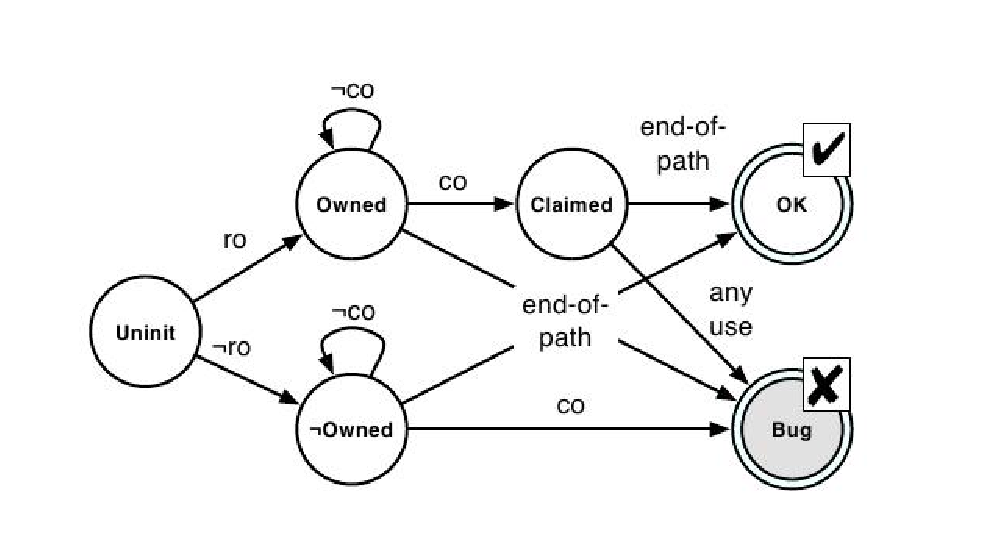
\includegraphics[scale=0.4]{fig.eps}
\caption{DFA summarizing basic ownership rules.}
\label{fig}
\end{figure}

Now let's define {\it annotation variables} for the example: {\it fopen:ret}, {\it fread:4} and {\it fclose:1}. The variable {\it fopen:ret} corresponds to the possible annotations for the return value of {\it fopen}, and has the domain $\{ro, \neg ro\}$. The variables {\it fread:4} and {\it fclose:1}(where :$i$ denotes the $i$th formal parameter) have the domain $\{co, \neg co\}$. We denote the set of annotation variables as $\mathbf{A}$. In our example, $\mathbf{A} = \{\textrm{{\it fopen:ret}, {\it fread:4}, {\it fclose:1}}\}$. Then we define factors in annotation factor graphs. Each factor $f_i$ is a map from the possible values of a set of variables $\mathbf{A}_i$($\mathbf{A}_i \subseteq \mathbf{A}$) to $[0, \infty)$. Factors ``score'' an assignment of values to a group of related annotation variables, with higher values indicating more belief in an assignment. We could define a {\it check} factor for our example, $f_{\langle check \rangle}(\textrm{{\it fopen:ret}, {\it fread:4}, {\it fclose:1}})$:
$$f_{\langle check \rangle}(\dots) = \left\{\begin{array}{ll} \theta_{\langle ok \rangle} & \textrm{if DFA = OK} \\ \theta_{\langle bug \rangle} & \textrm{if DFA = Bug} \end{array}\right..$$
Once we represent individual beliefs with factors, we combine a group of factors $\{f_j\}^J_{j=1}$ into a single probability model by multiplying their values together and normalizing:
$$P(\mathbf{A}) = \frac{1}{Z} \prod_{f_i\in \{f_j\}^J_{j=1}} f_i(\mathbf{A}_i).$$
The normalizing constant Z causes the scores to define a probability distribution over the values of A, which directly translates into a distribution over specifications. 

By using a more complicated DFA and introducing prior belief factors to indicate initial preferences, like $f_{\langle ro \rangle}$, they evaluated effectiveness of the framework on five codebases: SDL, OpenSSH, GIMP, and the OS kernels for Linux and Mac OS X(XNU). For each codebase, starting with zero initially provided annotations, they observed an inferred annotation accuracy of 80-90\%, with often near perfect accuracy for functions called as little as five times.

\paragraph{Strength}
The key strength of the approach is that it can incorporate many disparate forms of evidence. For instance, besides behavioral signatures and prior beliefs, we often have a volume of valuable, non-numeric ad hoc information such as domain-specific naming conventions (e.g., a function name containing the word ``alloc'' often implies the function is an allocator). Also the framework is pragmatic even for rapidly evolving codebases: the process of inferring annotations and using those annotations to check code with automated tools can be integrated into a nightly regression run. 

\paragraph{Weakness and Relation to Our Project}
The paper only applied their approach to the ownership problem. We don't know if it's also good for other specifications, like the interesting code efficiency problem in our project. Moreover essentially the paper is discussing the syntactical errors. However we are more interested in the semantical errors, that is whether the code could solve a particular problem. Although the syntactical error checking could rule out a lot of programms, it still remains unclear if the program could solve the particular problem or not. 
